\documentclass[tikz,border=6pt]{standalone}
\usepackage{tikz}
\usetikzlibrary{arrows.meta,positioning,calc}

%% fonts (same as before; optional)
\usepackage{dsfont}
\usepackage{newpxtext}
\usepackage{newpxmath}
\usepackage{amsmath}
\usepackage{caption}

% --- colors & styles (same palette) ---
\definecolor{incolor}{RGB}{255,194,120}   % soft orange
\definecolor{hidcolor}{RGB}{173,173,255}  % soft violet
\definecolor{outcolor}{RGB}{255,180,180}  % soft red

\def\noderad{8mm}     % matches minimum size=14mm → radius ~7mm; 9mm gives a nice stand-off
\def\scatter{0.2}     % tiny degrees; adjust 0.8–1.2 for more/less separation

\tikzset{
  nnnode/.style = {circle, minimum size=14mm, inner sep=0pt, font=\Large},
  inactive/.style = {nnnode, fill=gray!50},
  input/.style  = {nnnode, fill=incolor},
  hidden/.style = {nnnode, fill=hidcolor},
  output/.style = {nnnode, fill=outcolor},
  conn/.style   = {-{Stealth[length=2.5mm,width=2.0mm]},
                   line width=1pt, draw=gray!70},
  collabel/.style = {font=\Large, align=center}
}

\begin{document}
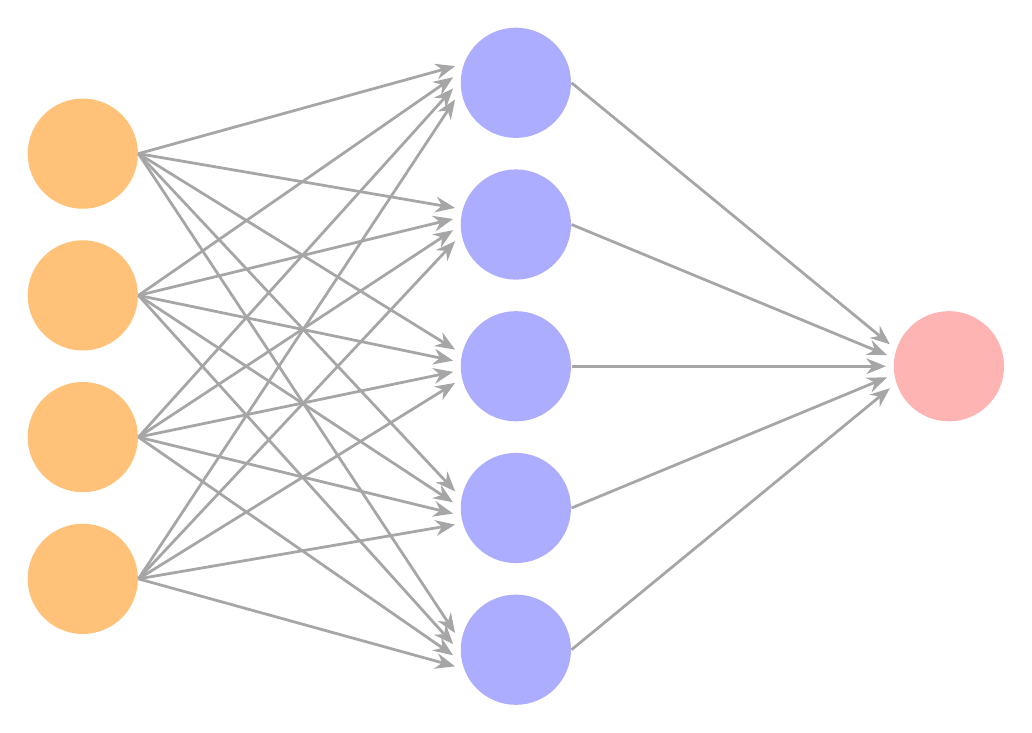
\begin{tikzpicture}[x=2.2cm,y=0.9cm]

% --- input layer (4 nodes) ---
\foreach \y/\name [count=\i] in {3/{$X_{1}$}, 1/{$X_{2}$}, -1/{$X_{3}$}, -3/{$X_{4}$}}{
  \node[input] (x\i) at (0,\y) {};
}

% --- hidden layer (5 nodes) ---
\foreach \y/\name [count=\j] in {4/{$A_{1}$}, 2/{$A_{2}$}, 0/{$A_{3}$}, -2/{$A_{4}$}, -4/{$A_{5}$}}{
  \node[hidden] (h\j) at (2.5,\y) {};
}

% --- output layer (single node) ---
\node[output] (out) at (5,0) {};

% --- connections: input -> hidden (STRAIGHT, tips slightly scattered) ---
\foreach \i [count=\m] in {1,...,4}{
  \foreach \j in {1,...,5}{
    \pgfmathsetmacro{\ang}{180 + (\m-2.5)*1\scatter} % scatter around west side
    \draw[conn] (x\i.east) -- ($(h\j)+(\ang:\noderad)$);
  }
}

% --- connections: hidden -> output (STRAIGHT, tips slightly scattered) ---
\foreach \j [count=\m] in {1,...,5}{
  \pgfmathsetmacro{\ang}{180 + (\m-3)*1\scatter}
  \draw[conn] (h\j.east) -- ($(out)+(\ang:\noderad)$);
}

\end{tikzpicture}

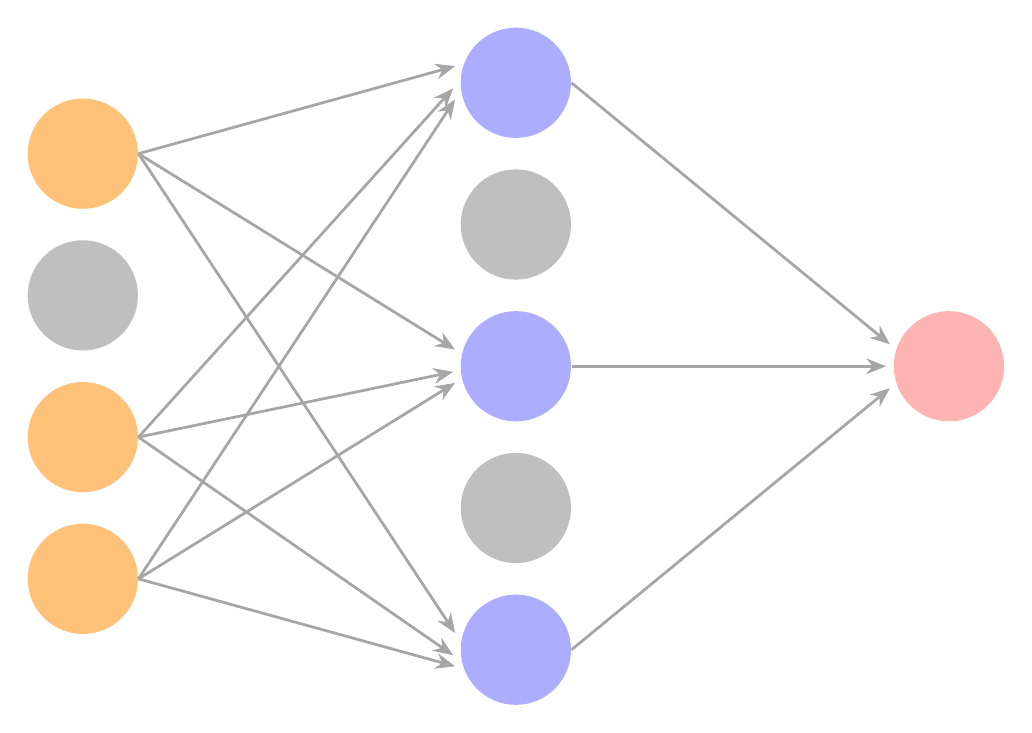
\begin{tikzpicture}[x=2.2cm,y=0.9cm]

% --- input layer (4 nodes), gray out #2 ---
\foreach \y/\name [count=\i] in {3/{$X_{1}$}, 1/{$X_{2}$}, -1/{$X_{3}$}, -3/{$X_{4}$}}{
  \ifnum\i=2
    \node[inactive] (x\i) at (0,\y) {};
  \else
    \node[input] (x\i) at (0,\y) {};
  \fi
}

% --- hidden layer (5 nodes), gray out #2 and #4 ---
\foreach \y/\name [count=\j] in {4/{$A_{1}$}, 2/{$A_{2}$}, 0/{$A_{3}$}, -2/{$A_{4}$}, -4/{$A_{5}$}}{
  \ifnum\j=2
    \node[inactive] (h\j) at (2.5,\y) {};
  \else
    \ifnum\j=4
      \node[inactive] (h\j) at (2.5,\y) {};
    \else
      \node[hidden] (h\j) at (2.5,\y) {};
    \fi
  \fi
}

% --- output layer ---
\node[output] (out) at (5,0) {};

% --- connections: input -> hidden (skip inactive) ---
\foreach \i [count=\m] in {1,...,4}{
  \foreach \j in {1,...,5}{
    \ifnum\i=2\else   % skip input #2
      \ifnum\j=2\else % skip hidden #2
        \ifnum\j=4\else % skip hidden #4
          \pgfmathsetmacro{\ang}{180 + (\m-2.5)*1\scatter}
          \draw[conn] (x\i.east) -- ($(h\j)+(\ang:\noderad)$);
        \fi
      \fi
    \fi
  }
}

% --- connections: hidden -> output (skip inactive) ---
\foreach \j [count=\m] in {1,...,5}{
  \ifnum\j=2\else
    \ifnum\j=4\else
      \pgfmathsetmacro{\ang}{180 + (\m-3)*1\scatter}
      \draw[conn] (h\j.east) -- ($(out)+(\ang:\noderad)$);
    \fi
  \fi
}

\end{tikzpicture}
\end{document}
